\documentclass[UTF8,fontset=fandol,11pt]{ctexart}

\usepackage[a4paper,margin=2.35cm]{geometry}
\usepackage{booktabs}
\usepackage{array}
\usepackage{tabularx}
\usepackage{graphicx}
\usepackage{float}
\usepackage{caption}
\usepackage{xcolor}
\usepackage{enumitem}
\usepackage{amsmath}
\usepackage{amssymb}
\usepackage{hyperref}

\definecolor{chapterblue}{HTML}{2F5F85}
\definecolor{softgray}{HTML}{F5F6F7}
\definecolor{textgray}{HTML}{333333}

\graphicspath{{../../charts/}}
\hypersetup{
  colorlinks=true,
  linkcolor=chapterblue,
  urlcolor=chapterblue,
  citecolor=chapterblue
}
\captionsetup{font=small,labelfont=bf}
\setlist[itemize]{leftmargin=1.6em,itemsep=0.15em}
\setlength{\parindent}{2em}
\setlength{\parskip}{0.35em}
\renewcommand{\arraystretch}{1.18}

\title{\textbf{第六部分：定量建模、状态依赖与风险扩展}}
\author{DASE7337 Group Project: Airline Delay and Cancellation Operational Risk}
\date{April 2026}

\begin{document}
\maketitle

\setcounter{section}{5}

\section{频率、严重度与模型选择}

\subsection{定量建模层的角色}
前一章节已经把原始 BTS 数据整理成了可直接建模的数据资产，并分别构造了 airline-month 和 airport-month 两层视角。本章节在此基础上进入风险测度阶段。整体逻辑仍然沿用课程中的标准框架：频率建模回答“扰动发生得有多频繁”，严重度建模回答“扰动一旦发生会造成多大的平均冲击”，状态依赖回答“高压力运行是否具有持续性”，年度 aggregate risk 模拟回答“这些因素在全年尺度上叠加后会形成怎样的风险分布”，而 EVT 与敏感度分析则进一步检验尾部解释与关键 driver 的稳健性。

本项目的损失口径并不是财务损失，而是以分钟为单位的 \textbf{delay-equivalent minutes}。原因其实很直接：BTS 原始数据直接记录的是延误分钟、取消和改降，而不是每次事件的现金损失。如果强行把分钟转换成货币，就必须额外引入一层成本假设。为了让“观测数据”与“建模对象”之间保持尽可能直接的对应关系，项目将运营冲击定义为分钟口径，并把整套框架定位为 operational-risk 模型，而不是 financial-loss 模型。

\subsection{为什么要比较候选分布}
项目并不预设某个变量一定服从某一种分布，而是先根据变量类型选出一组课程上合理的候选分布，再用统一标准进行比较。这样做有两个原因。第一，JFK 的运营数据同时包含平稳月份与高压月份，同一个变量完全可能呈现多种右偏或过度离散的形态。第二，项目的目标不仅仅是把一条曲线“拟合得更好”，而是要选出在统计上站得住、在运营上也解释得通的模型。

因此，对于频率变量，项目比较 Poisson 与 Negative Binomial；对于严重度变量，项目比较 Lognormal 与 Weibull。这种比较并不是随意增加方法，而是对应课程中“基准模型 vs 灵活模型”的思路：基准模型给出清晰的参考点，灵活模型则允许我们刻画机场运行中常见的聚集性、异质性和尾部放大效应。

\subsection{AIC：定义、作用与使用理由}
项目的模型选择采用 Akaike Information Criterion，即 AIC。其定义为
\[
\mathrm{AIC}=2k-2\log(\hat{L}),
\]
其中 \(k\) 为模型参数个数，\(\hat{L}\) 为参数估计完成后的最大似然值。

从直观上看，AIC 同时考虑两件事：一是模型对数据的拟合质量，二是模型本身的复杂度。如果一个模型只是因为参数更多而拟合得更好，AIC 会对这种复杂度进行惩罚。因此，AIC 越小，说明模型在“解释力”和“简洁性”之间的平衡越好。

这里需要特别说明，AIC 不是显著性检验，也不会给出 p-value。它的作用不是证明某个模型“显著正确”，而是在几个理论上都合理的候选模型之间，选出相对更优的那一个。这正是本项目需要的。我们面对的问题并不是“某个单一模型是否成立”，而是“在 Poisson 和 Negative Binomial 之间该选哪一个，在 Lognormal 和 Weibull 之间该选哪一个”。

相对于很多课程示例中更简单的比较思路，AIC 在本项目中有三个明显优势。第一，它可以比较非嵌套模型，因此非常适合 Lognormal 与 Weibull 这种结构不同但都合理的候选分布。第二，它会自动惩罚不必要的复杂度，避免模型只靠多参数取胜。第三，它为频率层和严重度层提供了一套统一的选择规则，使整个建模流程在方法上更一致、更可复现。也就是说，AIC 把课程中的 calibration 与 model verification 落成了一个明确、标准化的决策步骤。

因此，项目在每个变量上的模型选择都遵循同一流程：
\begin{enumerate}
  \item 先判断变量属于频率型还是严重度型；
  \item 为该变量选出课程上合理的候选分布；
  \item 用最大似然估计拟合各候选模型；
  \item 计算各候选模型的 AIC；
  \item 选择 AIC 更低的模型；
  \item 最后再从运营角度解释为什么这一选择是有意义的。
\end{enumerate}

\subsection{频率建模}
模型的第一层研究 airline-month 层面的计数型扰动变量。这里共对六个变量建模：总延误航班数、取消数、改降数、内部运营扰动计数、系统/NAS 扰动计数以及外部冲击扰动计数。这些变量天然属于课程中的 loss-number variables，因为它们回答的是“在固定的观察窗口内，扰动事件发生了多少次”。

Poisson 分布作为均匀到达的基准模型：
\[
\mathbb{P}(N=n)=e^{-\lambda}\frac{\lambda^n}{n!}, \qquad n=0,1,2,\dots
\]
在这个结构下，事件强度相对稳定，均值和方差接近。

Negative Binomial 分布则作为允许过度离散的灵活模型：
\[
\mathbb{P}(N=n)=\frac{\Gamma(n+r)}{\Gamma(r)\,n!}p^r(1-p)^n,
\qquad n=0,1,2,\dots
\]
这一模型允许方差显著大于均值，因此更适合刻画高压月份中事件成簇爆发的运营环境。

这一比较在运营上是有实质意义的。如果机场扰动真的接近 Poisson 过程，那么运营管理主要面对的是一个相对平稳的平均负荷；但如果扰动更接近 Negative Binomial，那么平均值本身就不够用了，系统还必须应对集中爆发、高压月份和运行脆弱性。

\begin{table}[H]
\centering
\caption{频率模型最终选择结果}
\begin{tabular}{lrrrr}
\toprule
变量 & 最终模型 & AIC & Normal 均值 & Disrupted 均值 \\
\midrule
总延误计数 & Negative Binomial & 7290.82 & 207.13 & 340.87 \\
取消计数 & Negative Binomial & 4463.27 & 14.15 & 84.36 \\
改降计数 & Negative Binomial & 2531.80 & 2.60 & 5.30 \\
内部运营计数 & Negative Binomial & 6766.28 & 132.65 & 204.68 \\
系统/NAS 计数 & Negative Binomial & 6047.51 & 68.42 & 124.20 \\
外部冲击计数 & Negative Binomial & 3502.99 & 6.06 & 12.00 \\
\bottomrule
\end{tabular}
\end{table}

结果非常一致：六个计数变量全部选中 Negative Binomial。这说明 JFK 的运营扰动并不是均匀随机分布在各个月份，而是具有明显的聚集性和压力积累效应。换句话说，机场运行并不是围绕一个稳定均值轻微波动，而是会进入少数高压力月份，在这些月份中多类扰动一起放大。

\begin{figure}[H]
\centering
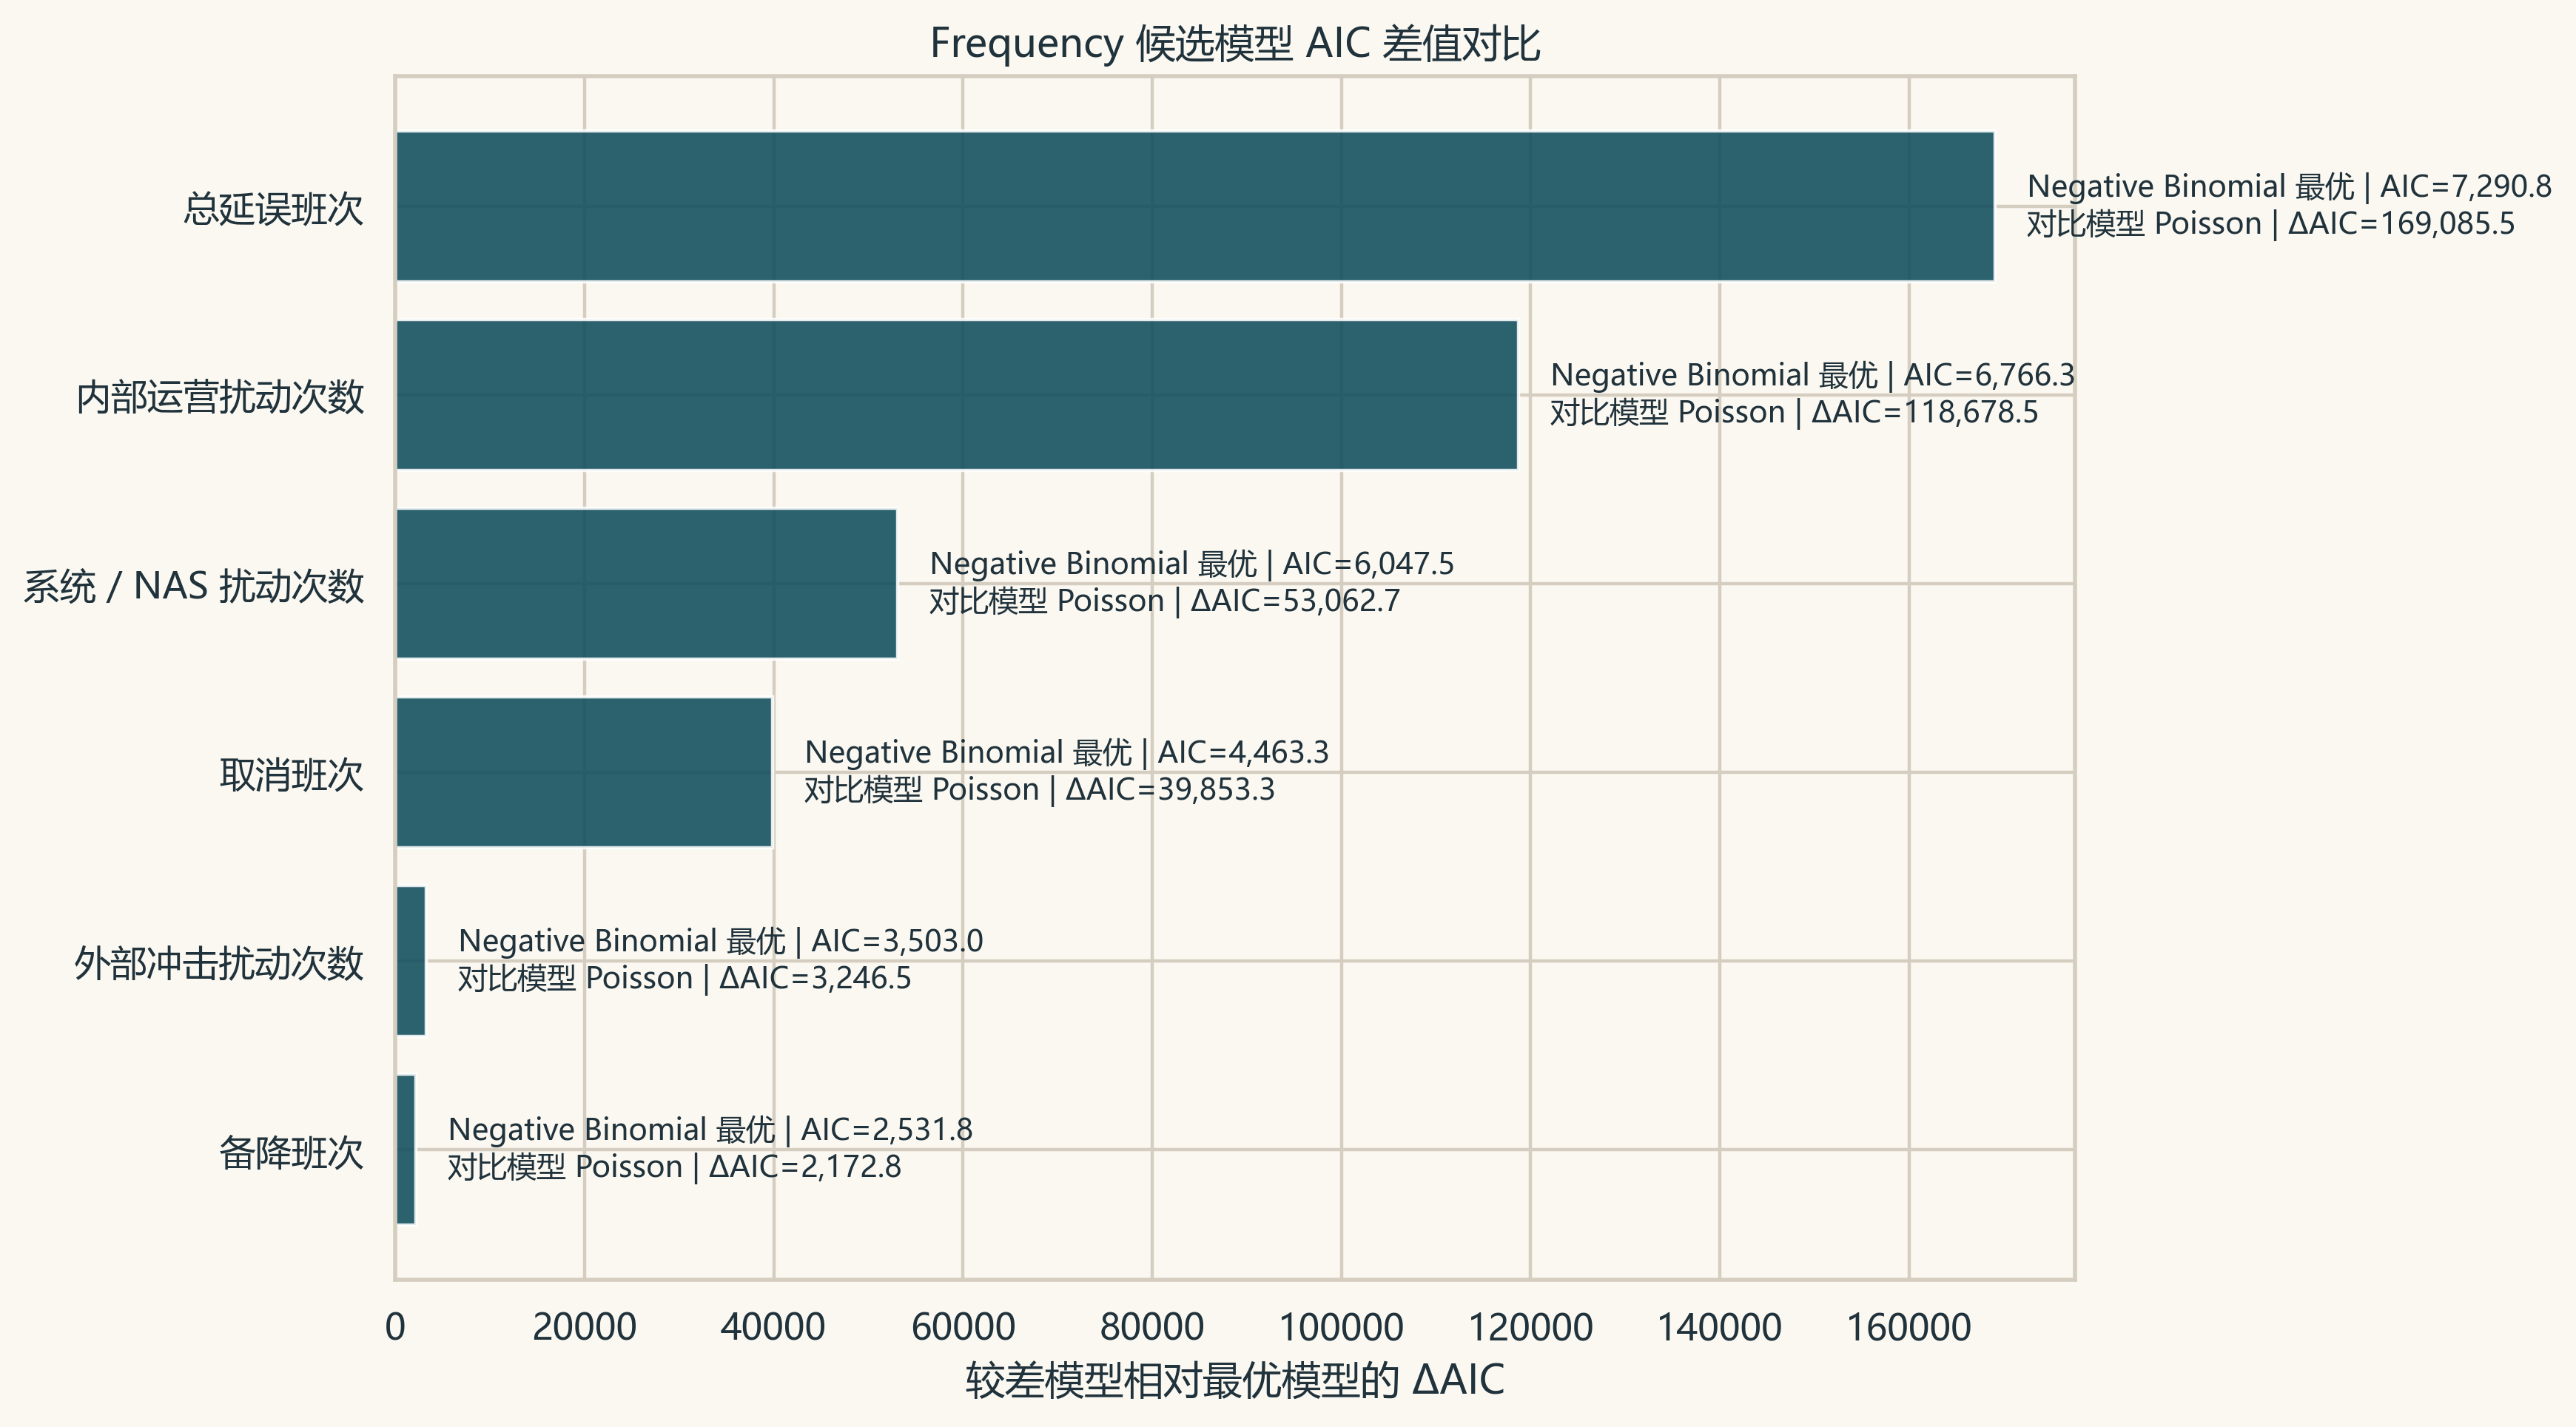
\includegraphics[width=0.92\linewidth]{chart_8_frequency_aic_comparison.png}
\caption{频率模型候选分布的 AIC 比较}
\label{fig:freq-aic-zh}
\end{figure}

图~\ref{fig:freq-aic-zh} 也把这一点直观地展示出来。对于每一个频率变量，Negative Binomial 的 AIC 都低于 Poisson。这意味着“扰动具有聚集性”不再只是直觉判断，而成为贯穿整个频率层的系统性结论。

\subsection{严重度建模}
模型的第二层研究扰动发生后的平均冲击大小。由于项目采用分钟口径，严重度定义为“每次扰动对应的平均延误分钟数”。这里建模的四个变量分别是：总体平均延误分钟、内部平均分钟、系统平均分钟和外部平均分钟。

第一类候选分布是 Lognormal：
\[
X \sim \mathrm{Lognormal}(\mu,\sigma^2)
\quad \Longleftrightarrow \quad
\log X \sim \mathcal{N}(\mu,\sigma^2).
\]
它适用于非负、右偏、且可能由多个乘法因素共同放大的损失过程。

第二类候选分布是 Weibull：
\[
f(x)=\frac{k}{\lambda}\left(\frac{x}{\lambda}\right)^{k-1}
e^{-(x/\lambda)^k}, \qquad x\ge 0.
\]
它同样适用于非负右偏变量，但在很多运营系统中更适合表示“尾部被现实约束拉长”的严重度模式。

比较这两种分布并不仅仅是统计层面的工作，也有清晰的运营解释。Lognormal 更像一类由多种摩擦因素叠加、逐步放大的冲击；Weibull 则更像一类仍然具有右尾，但受时刻表、机场容量、恢复机制等现实边界约束的冲击。

\begin{table}[H]
\centering
\caption{严重度模型最终选择结果}
\begin{tabular}{lrrrr}
\toprule
变量 & 最终模型 & AIC & Normal 均值 & Disrupted 均值 \\
\midrule
总体平均延误分钟 & Weibull & 5146.84 & 67.47 & 76.76 \\
内部平均分钟 & Lognormal & 5362.19 & 78.28 & 83.24 \\
系统平均分钟 & Lognormal & 4413.72 & 47.83 & 65.53 \\
外部平均分钟 & Lognormal & 4864.21 & 103.71 & 111.83 \\
\bottomrule
\end{tabular}
\end{table}

结果表明，总体严重度更适合 Weibull，而三类分块严重度都更适合 Lognormal。这个模式是合理的：在系统整体层面，平均冲击虽然有右尾，但仍然受到运营约束；在分块层面，内部、系统与外部风险更像是多重因素共同放大的右偏过程。

另一个重要发现是，所有严重度在 disrupted 状态下都高于 normal 状态，尤其 system/NAS 分块的增幅更明显。这说明高扰动月份不仅“更常出事”，而且“出了事也更重”。也正因为如此，后文才有必要把频率、严重度与状态依赖同时纳入年度 aggregate risk 模型。

\begin{figure}[H]
\centering
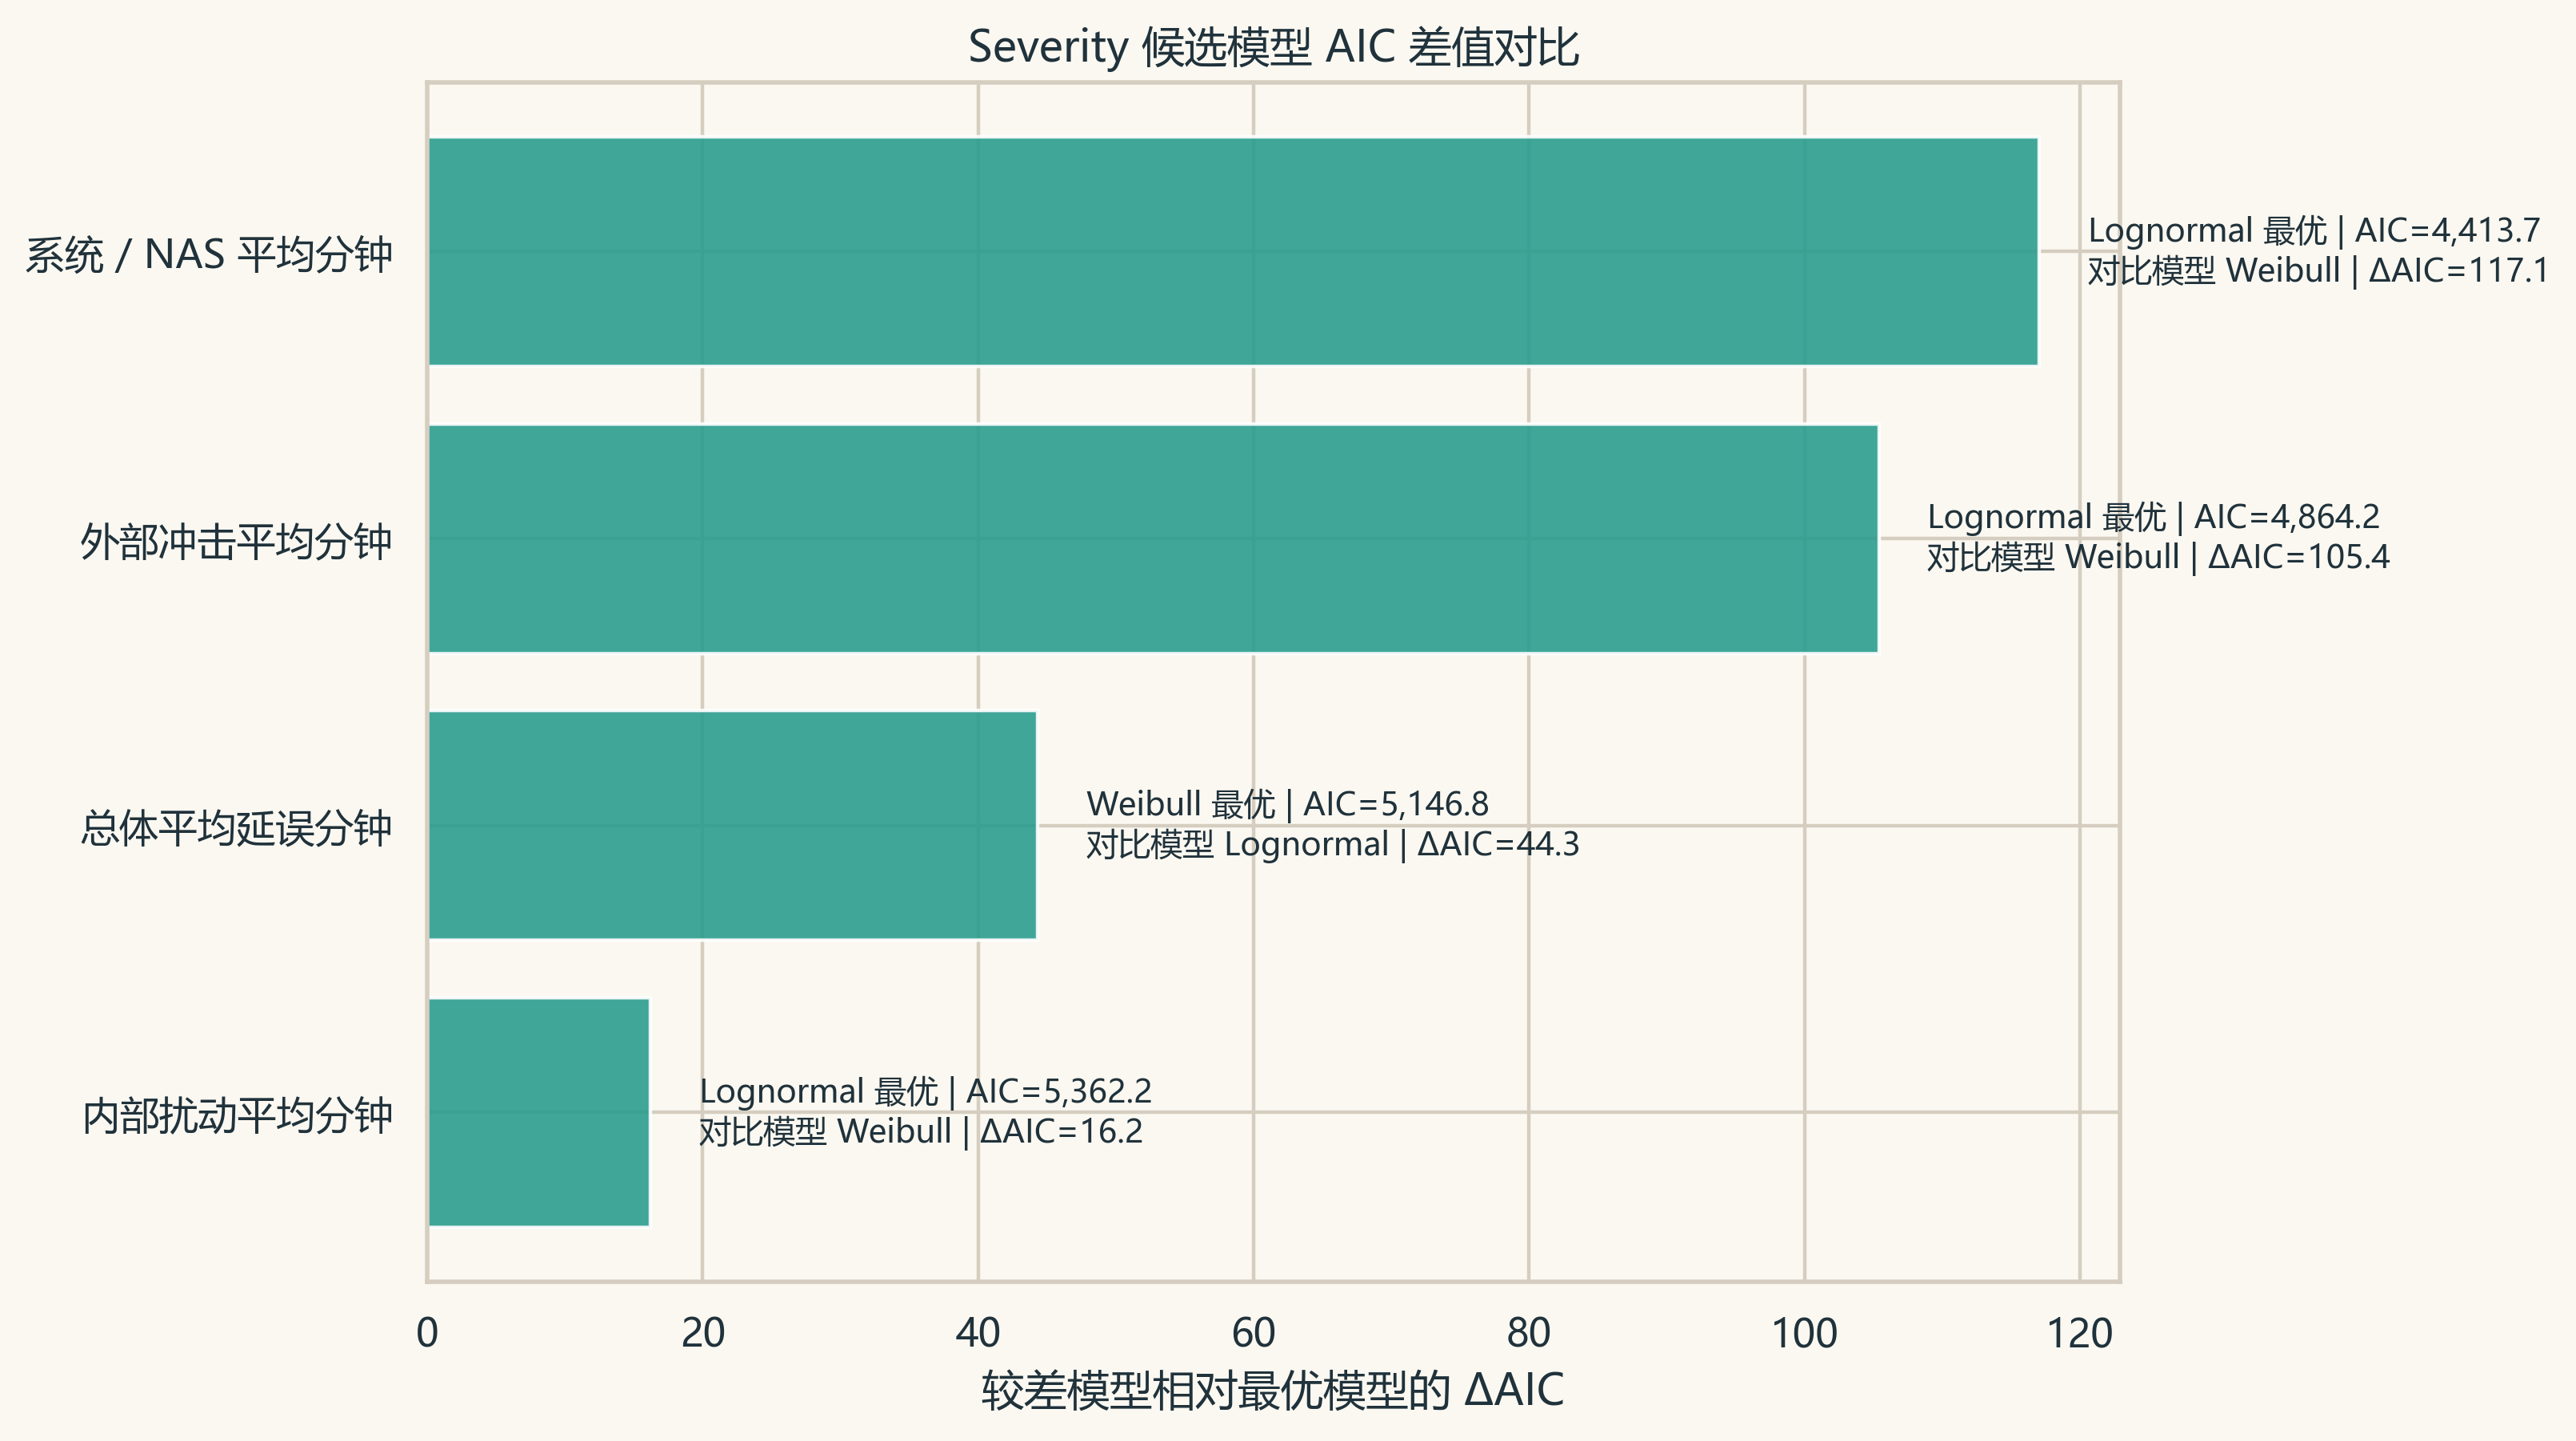
\includegraphics[width=0.92\linewidth]{chart_9_severity_aic_comparison.png}
\caption{严重度模型候选分布的 AIC 比较}
\label{fig:sev-aic-zh}
\end{figure}

\section{状态定义与 Markov 依赖}

\subsection{为什么需要状态依赖}
仅靠频率和严重度，还不足以刻画机场运行的动态过程。它们告诉我们“平均来说一个月会发生多少次扰动”和“每次扰动有多大”，但还没有回答“高压月份会不会持续”。现实中的机场运行并不会在每个月都自动回到一个完全中性的基线。高拥堵、高取消、累积延误与恢复压力，完全可能把系统推入连续多月的脆弱状态。因此，项目需要在 airport-month 层面增加一个状态层。

这里的状态设置刻意保持简洁，只区分两类：
\begin{itemize}
  \item \textit{Normal}
  \item \textit{Disrupted}
\end{itemize}
这样的设计不是为了穷尽机场运行的所有机制，而是为了回答本项目真正关心的问题：高压力运行状态是否存在持续性，以及这种持续性是否足以影响年度 aggregate risk。

\subsection{两种状态划分规则}
项目比较了两种 disrupted 月识别规则。第一种是单纯基于总冲击的阈值规则：
\[
\text{Disrupted}_t = \mathbf{1}\{ \text{Impact}_t \ge Q_{0.75}(\text{Impact}) \}.
\]
这一规则直观、透明，但只使用一个维度。

第二种是综合规则，将延误率、取消率和总运营冲击一起纳入：
\[
S_t = z(\text{DelayRate}_t) + z(\text{CancelRate}_t) + z(\text{Impact}_t),
\]
然后把综合分数位于样本前 25\% 的月份定义为 disrupted。

比较这两种规则的原因很直接。如果只看总冲击，那么状态容易被单一指标支配；如果同时看延误率、取消率和冲击总量，那么状态识别更接近“系统处于高压运行”的整体概念。最终选出的规则不能只靠直觉判断，还必须比较其跨年份稳定性。

\begin{table}[H]
\centering
\caption{候选 disrupted 规则的比较}
\begin{tabular}{lrrr}
\toprule
规则 & Disrupted 占比 & 年度标准差 & 是否选中 \\
\midrule
Impact 75\% 阈值规则 & 0.25 & 0.1863 & 否 \\
Delay-cancel-impact 综合规则 & 0.25 & 0.1521 & 是 \\
\bottomrule
\end{tabular}
\end{table}

最终选中的是综合规则。原因在于：两种规则都能保证整体上约 25\% 的月份被识别为 disrupted，但综合规则在不同年份之间更稳定。因此，它不仅在运营概念上更完整，在经验表现上也更平衡。

\subsection{为什么可以使用 Markov 链}
一旦定义了月度状态，下一步就是判断这些状态之间是否存在依赖。如果月份之间完全独立，那么“这个月是 disrupted”对“下个月是否 disrupted”就不应提供太多额外信息。反过来，如果高压力月份具有持续性，那么当前状态就应该能够帮助解释下个月的状态。这正是 Markov 链适用的情形。

项目采用一阶两状态 Markov 链，其转移概率定义为
\[
P_{ij}=\mathbb{P}(X_{t+1}=j \mid X_t=i),
\qquad i,j\in\{N,D\}.
\]
这里的目标不是构建一个高度复杂的隐状态模型，而是用最简洁的状态框架检验：机场运行是否存在可观测的 regime persistence。

\begin{table}[H]
\centering
\caption{两状态转移矩阵估计结果}
\begin{tabular}{llr}
\toprule
当前状态 & 下一状态 & 概率 \\
\midrule
Normal & Normal & 0.8148 \\
Normal & Disrupted & 0.1852 \\
Disrupted & Normal & 0.5294 \\
Disrupted & Disrupted & 0.4706 \\
\bottomrule
\end{tabular}
\end{table}

这里最关键的是 \(P(D\to D)\) 明显高于 \(P(N\to D)\)。也就是说，一旦系统进入高扰动状态，继续停留在高扰动状态的概率接近一半，而从正常状态转入高扰动状态的概率只有 18.5\%。这并不意味着我们已经完全识别了机场运行的深层机制，但它确实提供了有说服力的经验性证据：月度运行状态并非独立、无记忆地切换，而是存在持续性。

\begin{figure}[H]
\centering
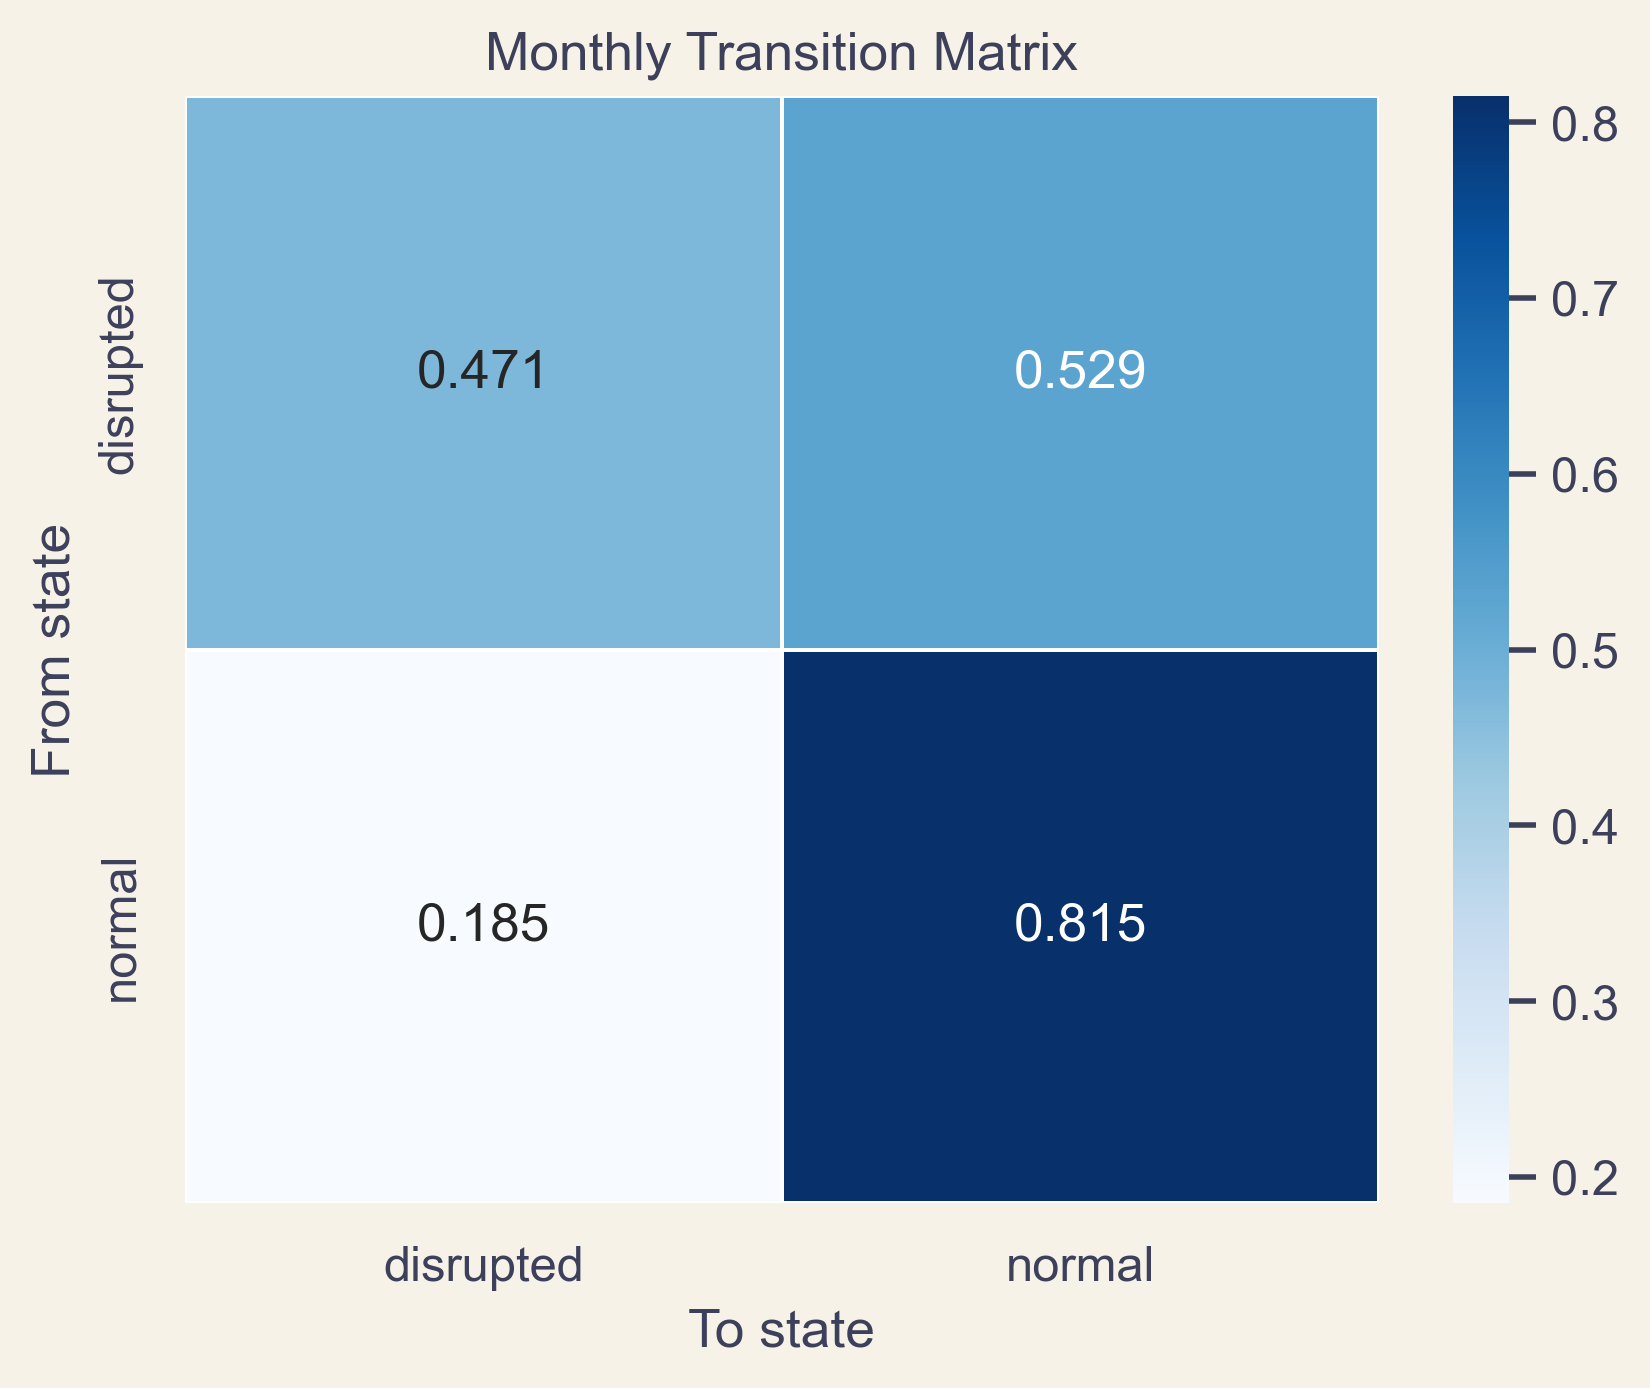
\includegraphics[width=0.52\linewidth]{chart_7_markov_transition_matrix.png}
\caption{两状态 Markov 转移矩阵}
\label{fig:markov-zh}
\end{figure}

因此，Markov 层为项目增加了一个频率和严重度本身无法提供的维度：它区分了“孤立的坏月份”和“会延续的高压运行阶段”。

\section{年度 Aggregate Risk 与 EVT 尾部扩展}

\subsection{从月度扰动到年度风险}
在频率、严重度与状态依赖都被建模之后，项目把它们合并成年度 aggregate operational risk。月度冲击定义为
\[
L_t = \text{DelayMinutes}_t + 180 \times \text{Cancelled}_t + 240 \times \text{Diverted}_t.
\]
然后把 12 个月的月度冲击相加得到年度总冲击：
\[
L^{(A)} = \sum_{t=1}^{12} L_t.
\]

这一步是整个项目的核心。因为在这之前，每个模型只解释了风险过程的一个部分；而年度模拟真正回答的是，这些因素叠加以后，全年会形成怎样的运营风险分布。这里要特别强调，项目并不是先模拟一个“代表性月份”再简单乘以 12，而是显式模拟一条完整的 12 个月路径：每个月先生成状态，再根据状态生成不同类型的扰动次数与严重度，最后把 12 个自然月的冲击累加成年度总风险。因此，这里的 annual risk 是路径型模拟结果，而不是静态放大结果。

更形式化地说，设 \(S_t \in \{N,D\}\) 表示第 \(t\) 个月的运行状态，其中 \(N\) 表示 Normal，\(D\) 表示 Disrupted。对于每一种扰动类型 \(j\)，其月度频率在给定状态下被模拟为
\[
N_{j,t}\mid S_t=s \sim F_j\!\left(\theta_j^{(s)}\right),
\]
其中 \(F_j\) 为已经选中的计数模型，即 Poisson 或 Negative Binomial。相应地，给定状态下的月度严重度被模拟为
\[
X_{j,t}\mid S_t=s \sim G_j\!\left(\phi_j^{(s)}\right),
\]
其中 \(G_j\) 为已经选中的严重度模型，即 Lognormal 或 Weibull。月度运营冲击由这些模拟出来的次数和严重度叠加取消与改降惩罚构成，而年度总冲击则是全部 12 个月冲击的和。

\subsection{情景设计}
项目在年度模拟中使用拟合得到的计数分布、严重度分布和状态转移结构，并设计了四个运营情景：
\begin{itemize}
  \item \textbf{Base}：基准运行环境；
  \item \textbf{Disruption Stress}：多类 driver 同时承压；
  \item \textbf{Holiday Peak}：高峰期运行压力上升；
  \item \textbf{Weather Shock}：外部冲击压力上升。
\end{itemize}

这些情景并不是对未来的逐月日历预测，也不意味着“全年 12 个月都处于某一种字面上的状态”。它们更准确的定位是：四种风格化的年度压力环境。每个情景都是在已经拟合好的频率层、严重度层和状态层之上，再叠加一组情景乘数，用来观察在不同压力模式下，全年风险分布会如何变化。

设 \(m^{(c,s)}_j\) 表示情景 \(c\) 下、状态 \(s\) 中作用于扰动 driver \(j\) 的频率乘数，\(q^{(c,s)}_j\) 表示对应的严重度乘数，则情景化后的模拟可写为
\[
\tilde{N}^{(c)}_{j,t} \sim F_j\!\left(\theta_j^{(S_t)}; m^{(c,S_t)}_j\right),
\qquad
\tilde{X}^{(c)}_{j,t} \sim G_j\!\left(\phi_j^{(S_t)}; q^{(c,S_t)}_j\right).
\]
也就是说，情景层并不是推翻前面的统计模型，而是在保留原有拟合结构的前提下，以一种可解释的方式对不同风险 driver 施加压力调整。

各个情景的实际含义，最好通过乘子设计来理解。Base 对应参考运行环境；Disruption Stress 表示多个风险 driver 同时被抬高；Weather Shock 重点抬高 external、cancel 和 divert；Holiday Peak 则表示一种更广义的旺季运行环境，在这种环境下，internal 周转压力、system 拥堵压力和 cancellation recovery 压力都会同步上升。换句话说，这四个情景描述的是四种不同的年度运行压力模式，而不是四个字面意义上的日历故事。为了让这一点更直观，表~\ref{tab:normal-multipliers-zh} 和表~\ref{tab:disrupted-multipliers-zh} 直接列出了正常状态与扰动状态下的情景乘子。

\begin{table}[H]
\centering
\caption{正常状态下的情景乘子}
\label{tab:normal-multipliers-zh}
\resizebox{\linewidth}{!}{
\begin{tabular}{lrrrrrrrr}
\toprule
Scenario & internal & system & external & cancel & divert & sev\_internal & sev\_system & sev\_external \\
\midrule
base & 1.00 & 1.00 & 1.00 & 1.00 & 1.00 & 1.00 & 1.00 & 1.00 \\
disruption\_stress & 1.05 & 1.10 & 1.10 & 1.05 & 1.05 & 1.03 & 1.05 & 1.05 \\
weather\_shock & 1.00 & 1.05 & 1.25 & 1.10 & 1.08 & 1.00 & 1.03 & 1.12 \\
holiday\_peak & 1.12 & 1.12 & 1.08 & 1.08 & 1.05 & 1.05 & 1.05 & 1.03 \\
\bottomrule
\end{tabular}
}
\end{table}

\begin{table}[H]
\centering
\caption{扰动状态下的情景乘子}
\label{tab:disrupted-multipliers-zh}
\resizebox{\linewidth}{!}{
\begin{tabular}{lrrrrrrrr}
\toprule
Scenario & internal & system & external & cancel & divert & sev\_internal & sev\_system & sev\_external \\
\midrule
base & 1.10 & 1.20 & 1.25 & 1.15 & 1.10 & 1.05 & 1.08 & 1.10 \\
disruption\_stress & 1.25 & 1.35 & 1.45 & 1.30 & 1.20 & 1.10 & 1.15 & 1.20 \\
weather\_shock & 1.05 & 1.15 & 1.65 & 1.40 & 1.30 & 1.02 & 1.08 & 1.25 \\
holiday\_peak & 1.22 & 1.28 & 1.18 & 1.22 & 1.15 & 1.10 & 1.12 & 1.08 \\
\bottomrule
\end{tabular}
}
\end{table}

这样看，情景分析的作用就会更清楚。它回答的是一个比较性问题：如果全年运行环境更像这些压力模式之一，那么 annual loss distribution 会如何变化？重点并不是去讲一个逐月展开的字面日历故事，而是用一组结构化乘子去测试不同压力模式下年度风险分布的反应程度，而乘子表本身就把这种差异直接展示出来了。

\begin{table}[H]
\centering
\caption{各情景下的年度 aggregate operational impact}
\begin{tabular}{lrrrrr}
\toprule
情景 & Expected & VaR95 & TVaR95 & VaR99 & TVaR99 \\
\midrule
Base & 2,348,090 & 2,783,840 & 2,907,633 & 2,987,687 & 3,091,504 \\
Disruption Stress & 2,611,485 & 3,113,791 & 3,265,407 & 3,356,033 & 3,488,504 \\
Holiday Peak & 2,672,771 & 3,161,531 & 3,307,414 & 3,400,303 & 3,519,168 \\
Weather Shock & 2,464,786 & 2,915,166 & 3,043,597 & 3,124,134 & 3,238,526 \\
\bottomrule
\end{tabular}
\end{table}

年度结果首先展示出 Base 与三个压力情景之间的明显差距。三种压力情景都会抬高 expected impact 和 tail metrics，但抬高的机制并不相同。Disruption Stress 和 Holiday Peak 的整体上升更明显，这与它们在 internal、system 和 cancellation-related driver 上更广泛的乘子抬升一致；Weather Shock 也会显著推高年度风险，但它的影响更集中在 external、cancel 和 divert 相关通道。这个比较的重要性在于，它说明年度风险并不只来自孤立的外部冲击，也来自多类运营压力在全年反复出现时形成的系统性放大。

从风险度量的角度，设 \(L^{(A,c)}\) 表示情景 \(c\) 下的年度总冲击，则项目报告的关键指标包括
\[
\mathrm{VaR}_{\alpha}\!\left(L^{(A,c)}\right)
=
\inf \left\{ \ell : \mathbb{P}\!\left(L^{(A,c)} \le \ell\right)\ge \alpha \right\},
\]
以及
\[
\mathrm{TVaR}_{\alpha}\!\left(L^{(A,c)}\right)
=
\mathbb{E}\!\left[L^{(A,c)} \mid L^{(A,c)}>\mathrm{VaR}_{\alpha}\!\left(L^{(A,c)}\right)\right].
\]
这些指标之所以重要，是因为它们不仅描述年度风险分布的中心位置，也刻画了极端年份中的平均冲击水平，因此特别适合比较不同年度压力情景之间的尾部差异。

\begin{figure}[H]
\centering
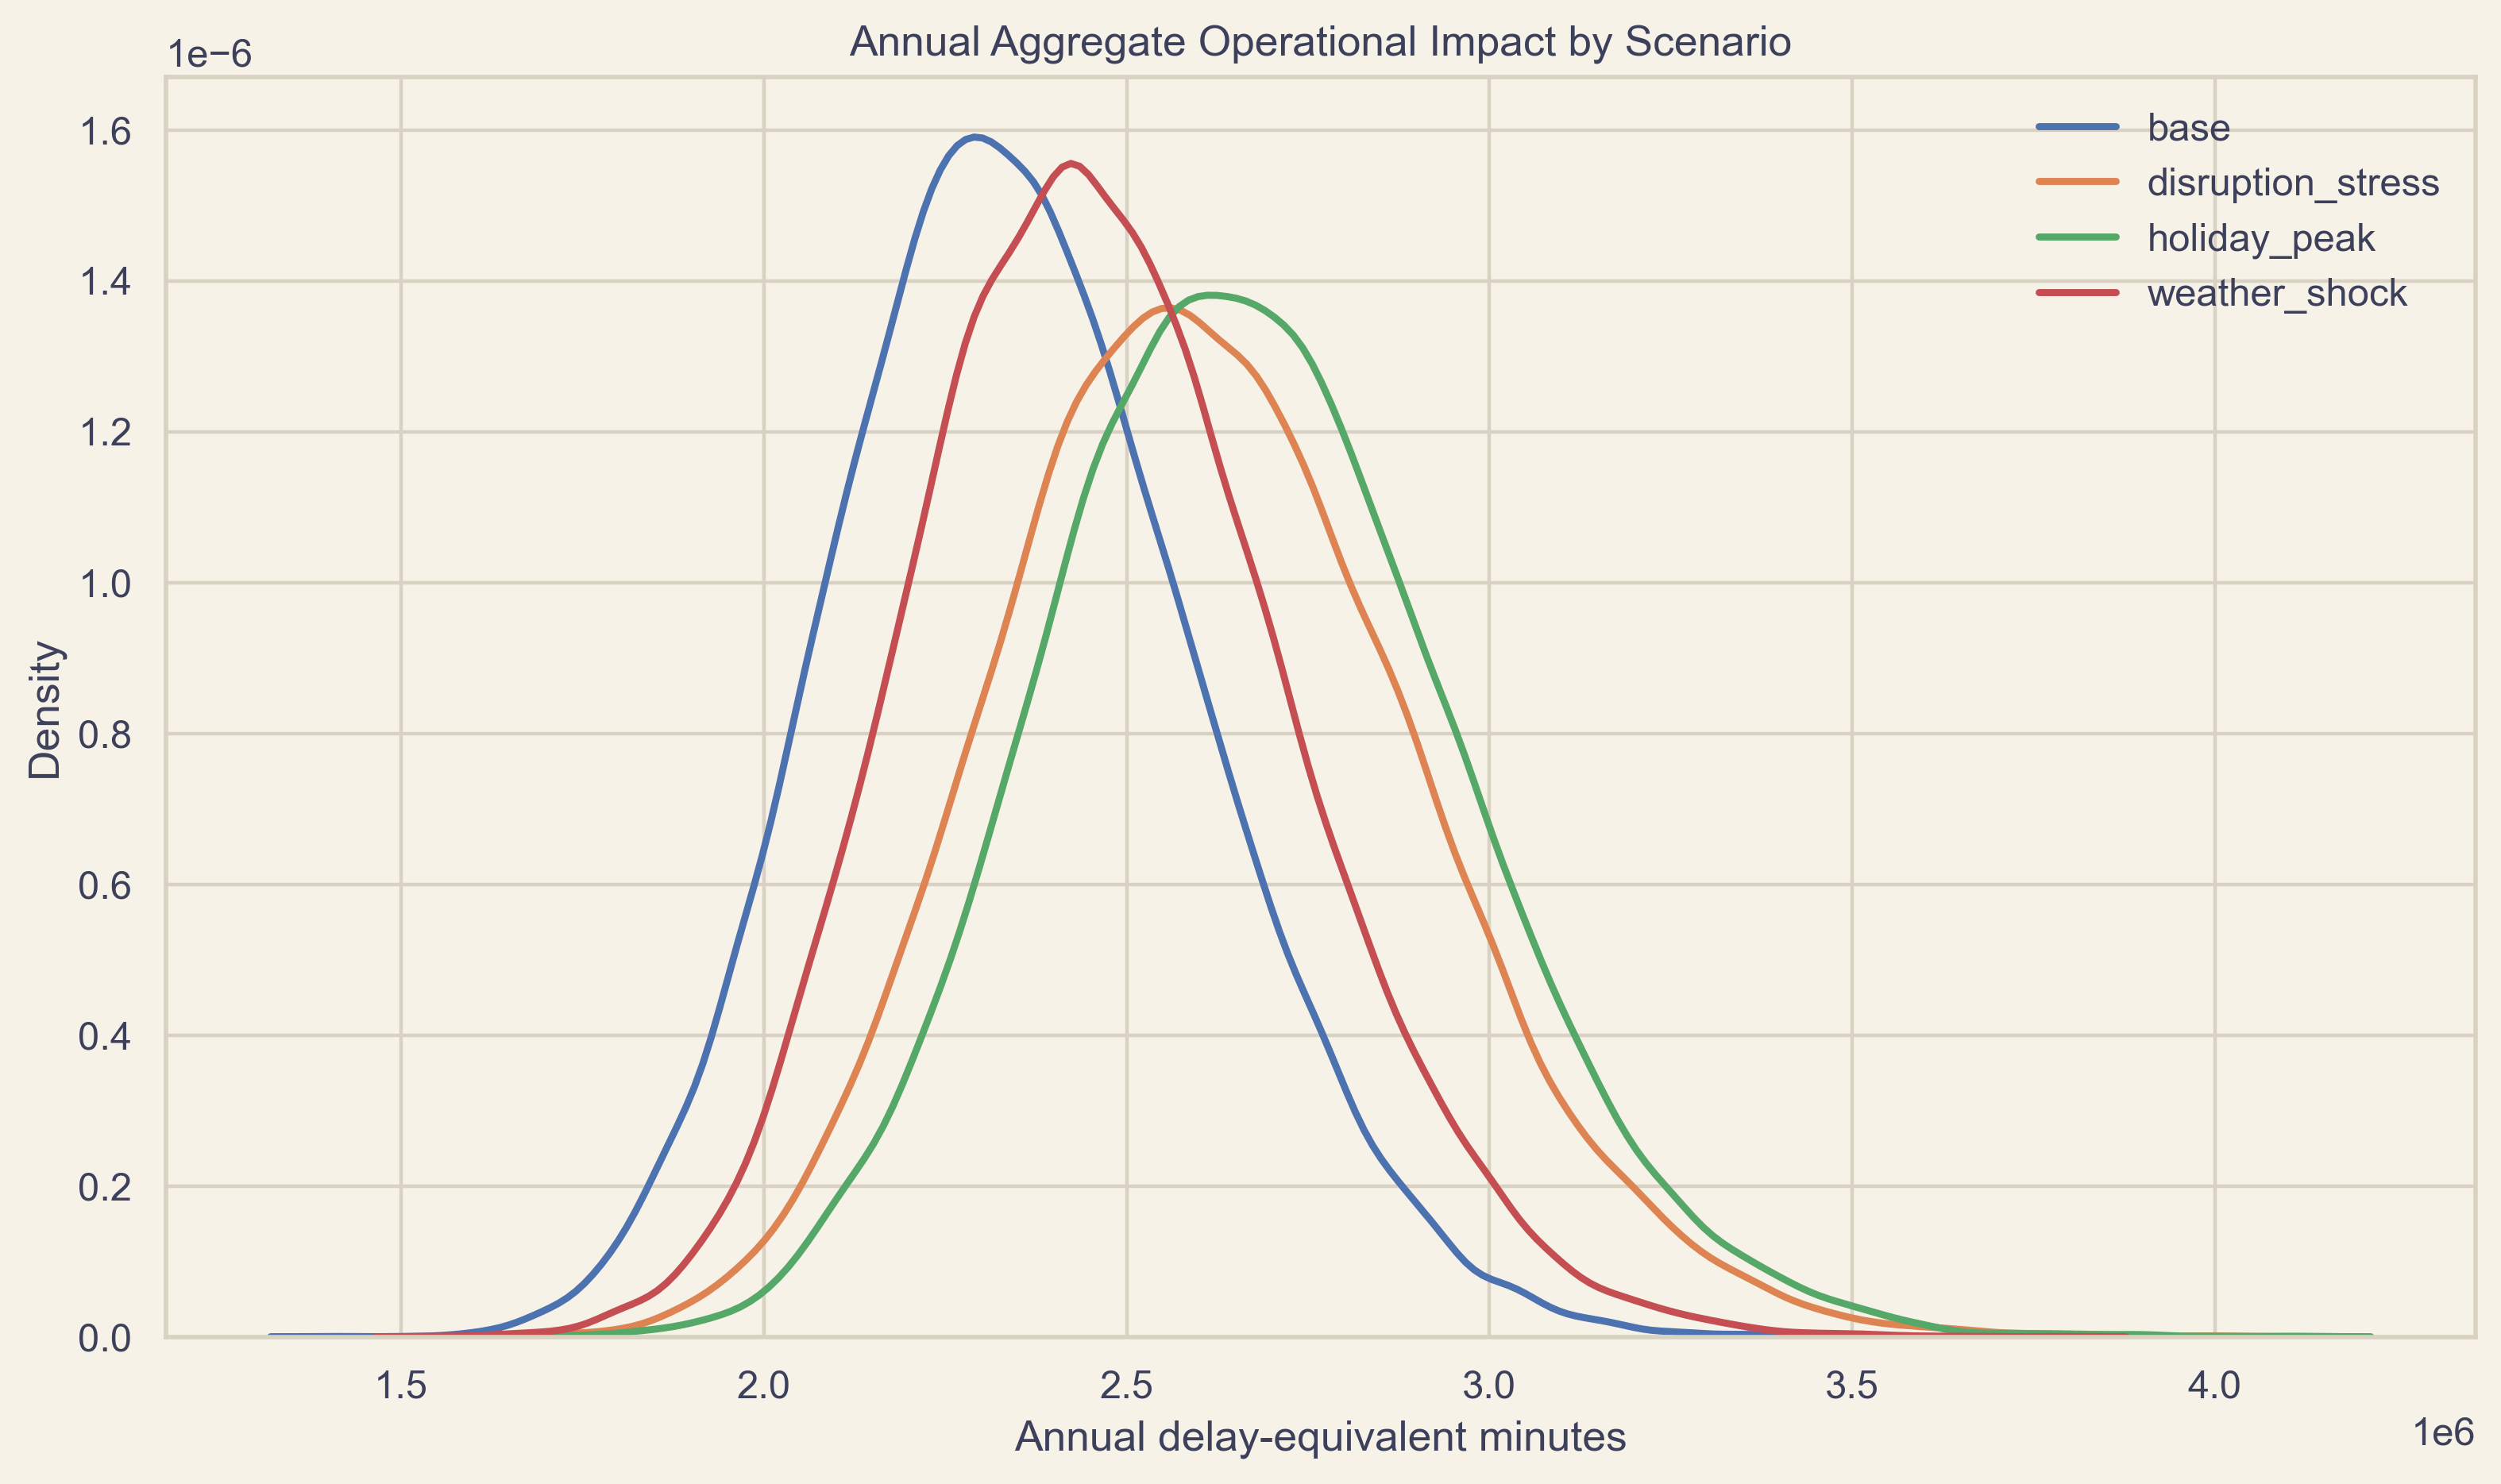
\includegraphics[width=0.90\linewidth]{chart_6_aggregate_risk_scenarios.png}
\caption{不同情景下的年度 aggregate risk 分布}
\label{fig:agg-risk-zh}
\end{figure}

\subsection{EVT 尾部扩展}
由于年度运营风险最重要的部分往往集中在尾部，项目在 annual aggregate impact 上进一步加入 EVT 扩展，采用 peaks-over-threshold 方法。设年度总冲击为 \(L\)，取较高阈值 \(u\)，则超额量定义为
\[
Y=L-u \mid L>u.
\]
在阈值之上，超额量服从 Generalized Pareto Distribution:
\[
\mathbb{P}(Y\le y)=1-\left(1+\xi \frac{y}{\beta}\right)^{-1/\xi},
\qquad y>0.
\]
其中 \(\xi\) 为 shape parameter，\(\beta\) 为 scale parameter。

项目默认使用年度模拟结果的 95\% 分位数作为阈值，并进一步做阈值敏感度分析。这里 EVT 的定位不是替代主模拟框架，而是作为尾部解释层，对主模型的极端风险结论进行增强和检验。

\begin{table}[H]
\centering
\caption{EVT 尾部拟合结果摘要}
\begin{tabular}{lrrrr}
\toprule
情景 & Shape \(\xi\) & Scale \(\beta\) & Empirical TVaR99 & EVT TVaR99 \\
\midrule
Base & -0.0833 & 134,061 & 3,091,504 & 3,094,013 \\
Disruption Stress & -0.0898 & 165,189 & 3,488,504 & 3,492,498 \\
Holiday Peak & -0.0873 & 158,518 & 3,519,168 & 3,526,243 \\
Weather Shock & -0.0856 & 139,435 & 3,238,526 & 3,236,719 \\
\bottomrule
\end{tabular}
\end{table}

这里可以得到两个结论。第一，四个情景下的形状参数 \(\xi\) 都为负，说明尾部虽然偏重，但不是爆炸式厚尾。第二，经验 TVaR99 与 EVT TVaR99 在各情景下都非常接近，说明主模拟本身给出的尾部刻画已经相当稳定，EVT 更多起到验证和增强作用，而不是推翻主模型。

\section{敏感度分析}

\subsection{为什么还需要敏感度分析}
年度 aggregate risk 与 EVT 已经给出了尾部风险的总体图景，但管理层还需要知道：到底哪些 driver 最值得优先控制。敏感度分析就是为了回答这个问题。它通过对关键风险因子施加目标冲击，观察年度 expected impact 和 tail metrics 的变化幅度，从而识别最重要的风险驱动因素。

在运营风险项目中，这一步尤其重要，因为不同 driver 的管理含义并不一样。有些风险重要，是因为发生频繁；有些重要，是因为单次冲击很大；还有一些重要，是因为它们对尾部风险具有放大作用。敏感度分析就是用来区分这些角色的。

\subsection{敏感度设计}
项目同时考虑了单因子冲击与组合冲击。单因子情景分别提高 internal、system、external、cancel 和 divert 等 driver；组合情景则测试多个风险因子同时抬升时，尾部风险是否被共同放大。

为便于解释，项目把每个情景的结果都写成相对于 Base 的百分比变化：
\[
\%\Delta = \frac{\text{Metric}_{\text{shock}}-\text{Metric}_{\text{base}}}{\text{Metric}_{\text{base}}}\times 100.
\]
这里的指标不仅包括 expected annual impact，也包括 empirical TVaR99 和 EVT TVaR99。

\begin{table}[H]
\centering
\caption{对 EVT TVaR 99\% 提升最大的敏感度情景}
\begin{tabular}{lrrr}
\toprule
情景 & Expected 变化 & TVaR99 变化 & EVT TVaR99 变化 \\
\midrule
Internal +30\% & 15.15\% & 16.21\% & 16.24\% \\
Internal + Cancel +20\% & 14.86\% & 15.22\% & 15.27\% \\
Internal + System +20\% & 13.77\% & 13.71\% & 13.90\% \\
Internal +20\% & 10.20\% & 10.83\% & 10.91\% \\
Cancel +30\% & 6.62\% & 7.42\% & 7.45\% \\
\bottomrule
\end{tabular}
\end{table}

敏感度结论相当清楚。最强的 driver 是 internal operational disruption，其次是 cancellation amplification。相比之下，diversion-only 冲击的影响明显更弱。这样一来，项目就不再只是停留在“量化风险”这一步，而是能够进一步支持管理决策：最值得优先控制的是飞机周转韧性、周转缓冲、机组与维护协调，以及取消后的恢复能力。

\begin{figure}[H]
\centering
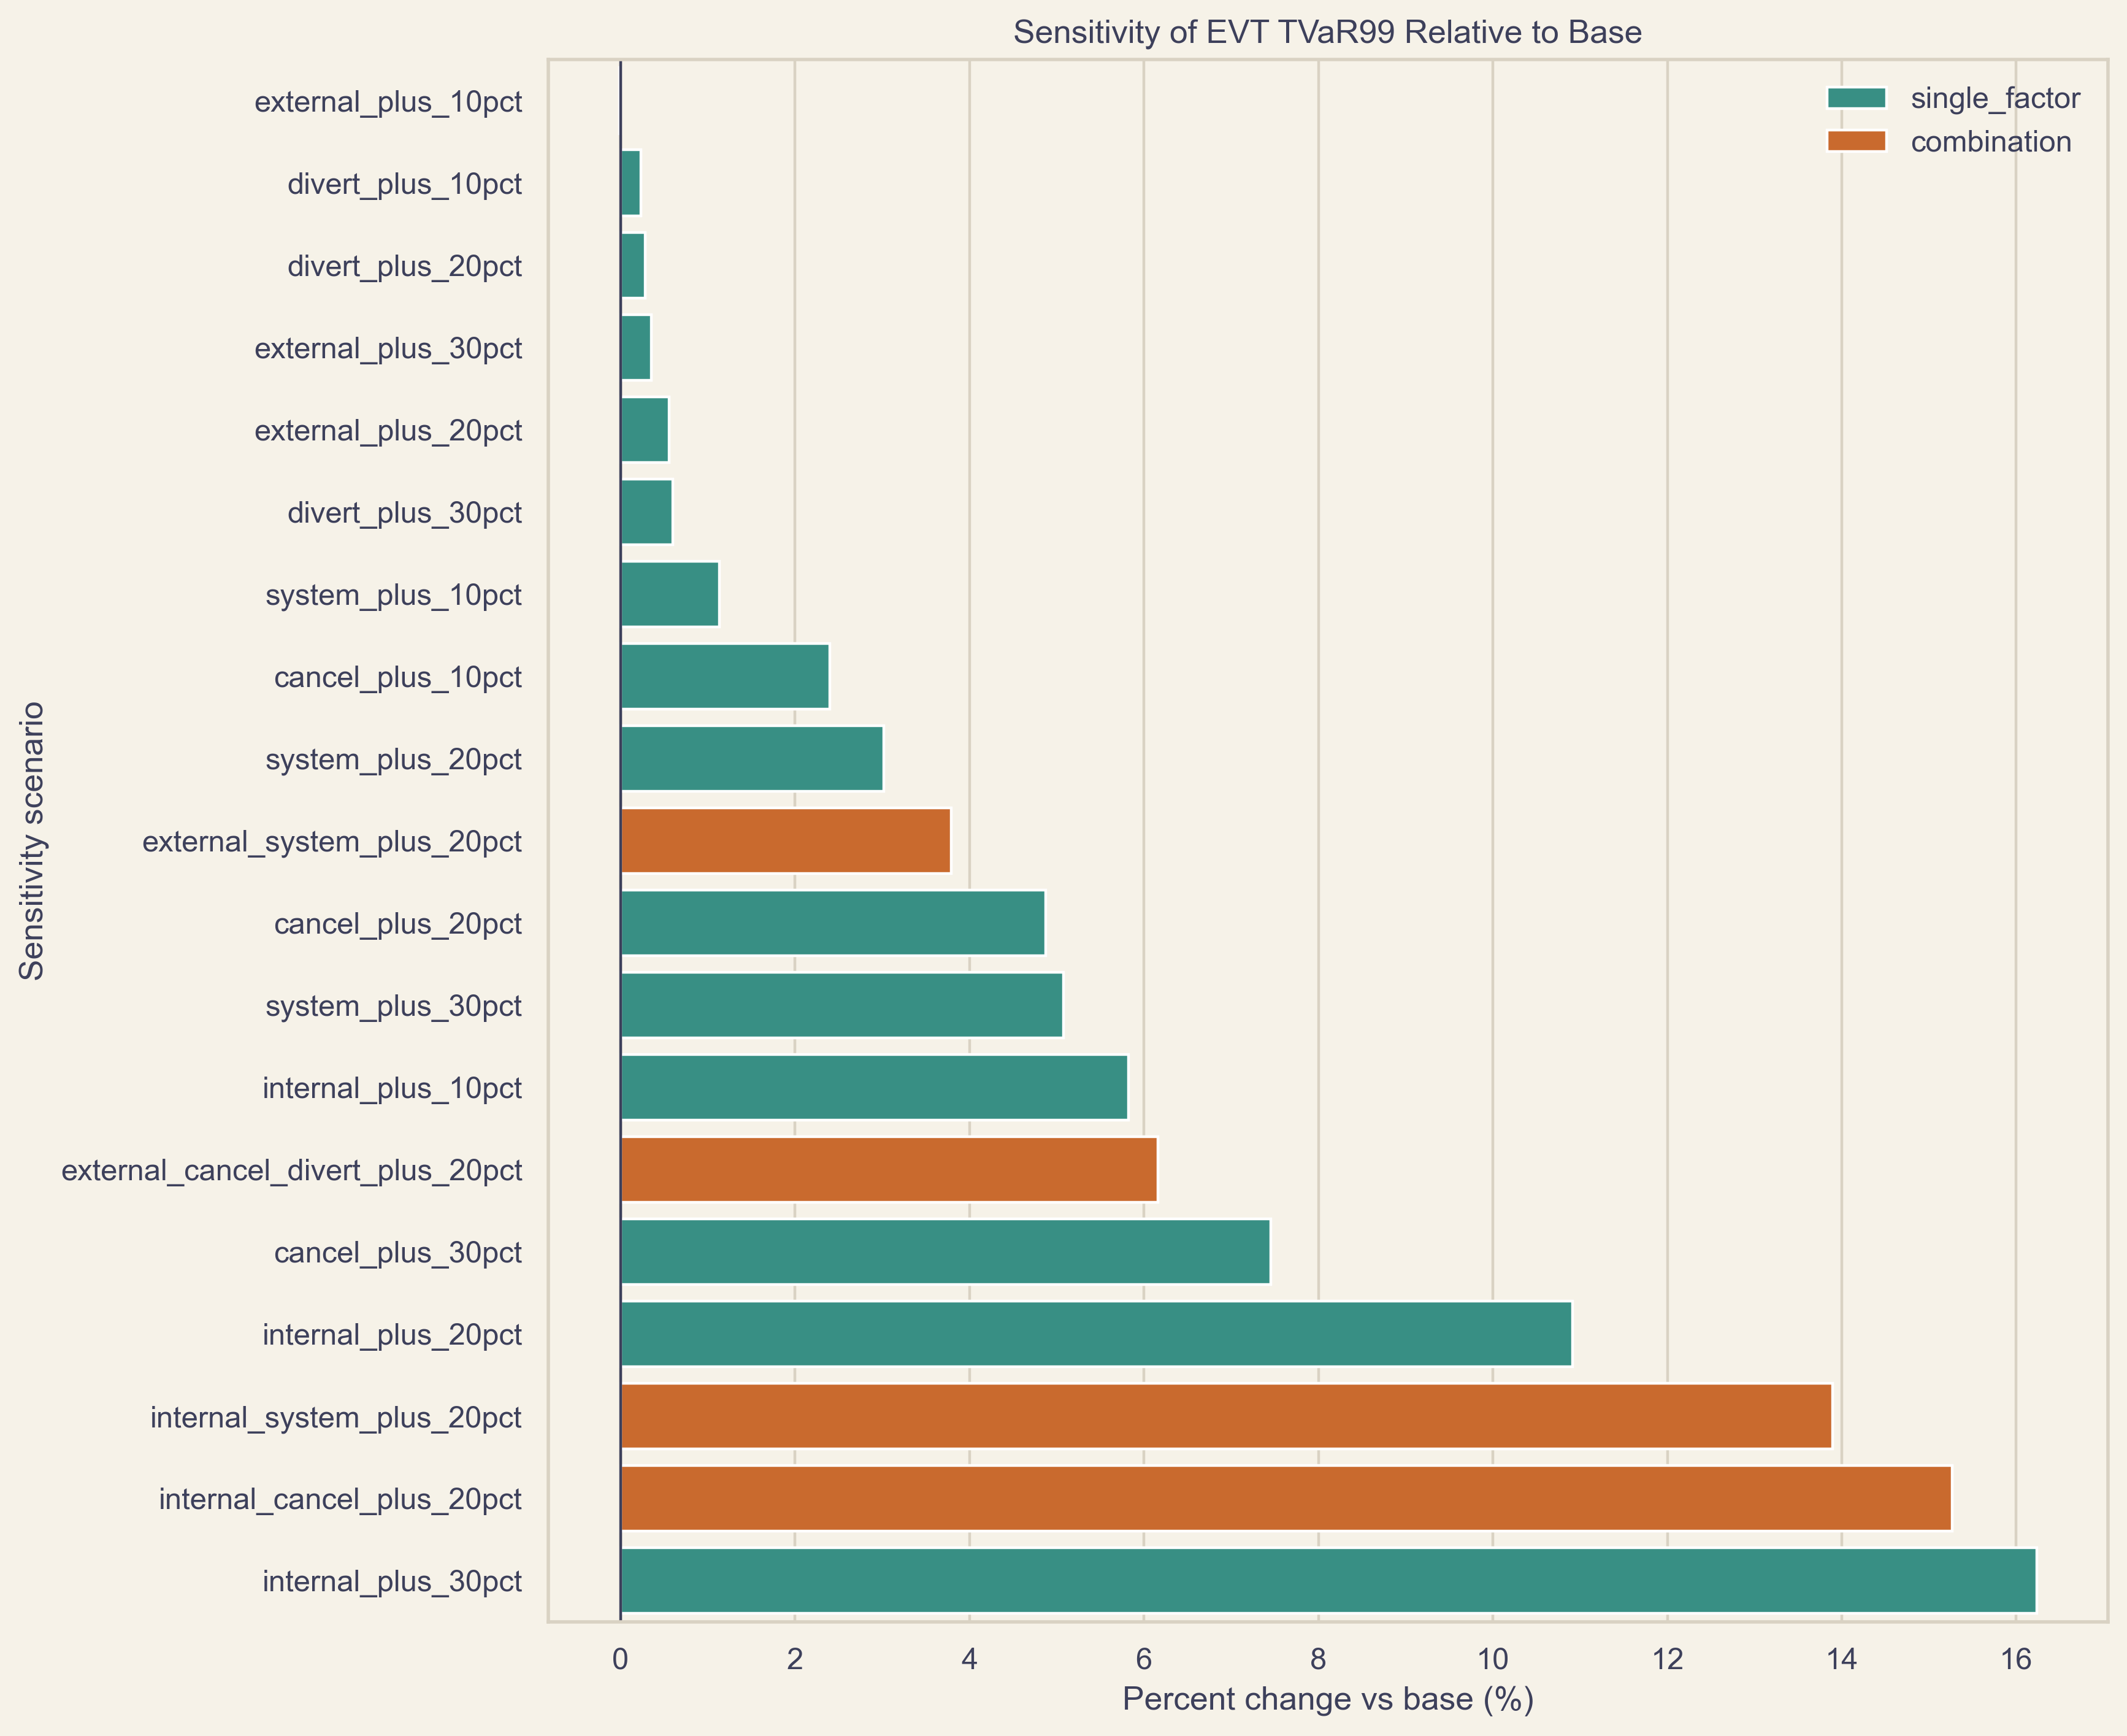
\includegraphics[width=0.90\linewidth]{chart_13_sensitivity_tornado.png}
\caption{相对于 Base 的 EVT TVaR 99\% 敏感度结果}
\label{fig:sensitivity-zh}
\end{figure}

\section{综合解释与局限}
将以上各层结果合在一起看，项目形成了一条比之前更完整的风险叙事。第一，扰动频率不是均匀随机发生，而是具有明显聚集性，因此 Negative Binomial 在频率层中全面胜出。第二，严重度是右偏的，而且在 disrupted 状态下更高，这说明高扰动月份不仅事件更多，而且单次冲击更重。第三，月度运行状态具有持续性，因此使用两状态 Markov 结构来描述依赖是有根据的。第四，年度 aggregate risk 更受广义高压运行环境和旺季压力驱动，而不只是受孤立天气事件驱动。第五，EVT 检验与敏感度分析共同说明，尾部风险结论总体稳定，而内部运营链条与取消恢复能力是最值得优先管理的 driver。

当然，这一章节也有几个需要诚实说明的局限。第一，损失口径仍然是分钟 proxy，而不是观测到的财务损失。第二，两状态 regime 结构是刻意保持简洁的近似框架，适合课程项目，但不应被解释为对机场运行机制的完全刻画。第三，EVT 的有效性依赖于基础模拟结果，因此它是主模型上的尾部扩展，而不是独立于主模型之外的新模型。

即便存在这些局限，这一章节也已经不仅仅是在罗列结果，而是在更完整地说明：模型为什么这样设计、每一层到底回答了什么问题、为什么选用这些方法、这些结果又意味着什么。对于后续最终报告的讨论、结论和答辩，这样的结构会更稳，也更像一份完整的定量风险报告。

\end{document}
